\documentclass[10pt]{beamer}

\input{/Users/daniel/Documents/LaTeX/beamer-style.tex}

\title{SGBD - 2\textsuperscript{e}}
\subtitle{PL-SQL - Chapitre 1 - Généralités}
\date{\today}
\author{Daniel Schreurs}
\institute{Haute École de Province de Liège}
%\titlegraphic{\hfill\includegraphics[height=1.5cm]{logo.eps}}

\setbeamertemplate{frame footer}{\insertsectionhead}
\begin{document}
\maketitle

\setbeamerfont{subsection in toc}{size=\small}
\setbeamerfont{subsubsection in toc}{size=\normalsize}
\setbeamertemplate{section in toc}[sections numbered]
\setbeamertemplate{subsection in toc}[subsections numbered]
\setbeamertemplate{subsubsection in toc}[subsubsections numbered]
\begin{frame}[allowframebreaks]{Table des matières du chapitre}
    \tableofcontents[subsectionstyle=show/show/hide,subsubsectionstyle=show/show/hide,]
\end{frame}

\section{Introduction}
\tocss
\subsection{Définition}
\begin{frame}{\secname : \subsecname}
    \begin{itemize}
        \item PL/SQL : Procedural Language extensions to SQL;
        \item PL/SQL est un langage procédural qui permet de traiter de manière structurée (conditionnelle ou itérative) les données retournées par une instruction SQL;
        \item Il s'agit d'un langage propriétaire, PL/SQL est la solution proposée par Oracle.
    \end{itemize}
\end{frame}

\begin{frame}{\secname : \subsecname}
    \begin{itemize}
        \item Au niveau syntaxe, un programme est constitué de procédures et de fonctions; des variables permettent l'échange d'information entre les requêtes SQL et le reste du programme.
        \item \textbf{PL/SQL n'a aucun aspect normatif} contrairement à SQL.\footnote{Mais avec SQL3, la norme SQL a prévu les éléments de langage procédural normatif propre au langage SQL.}
              PL/SQL permet de \textbf{stocker du code sur le serveur} et sert principalement à \textbf{programmer des procédures stockées} et \textbf{des déclencheurs} (triggers)
    \end{itemize}
\end{frame}
\section{PL/SQL}
\subsection{Pourquoi}

\begin{frame}{\secname : \subsecname}
    Meilleure performance en écrivant des blocs de programmation PL/SQL :
    \begin{itemize}
        \item Les ordres SQL ne sont plus transmis un à un au moteur de base de données Oracle mais par bloc de programmation        moins de trafic réseau
        \item Le moteur PL/SQL a été optimisé ce qui améliore encore les performances globales des applications
    \end{itemize}
\end{frame}

\begin{frame}{\secname : \subsecname}
    \begin{figure}
        \begin{center}
            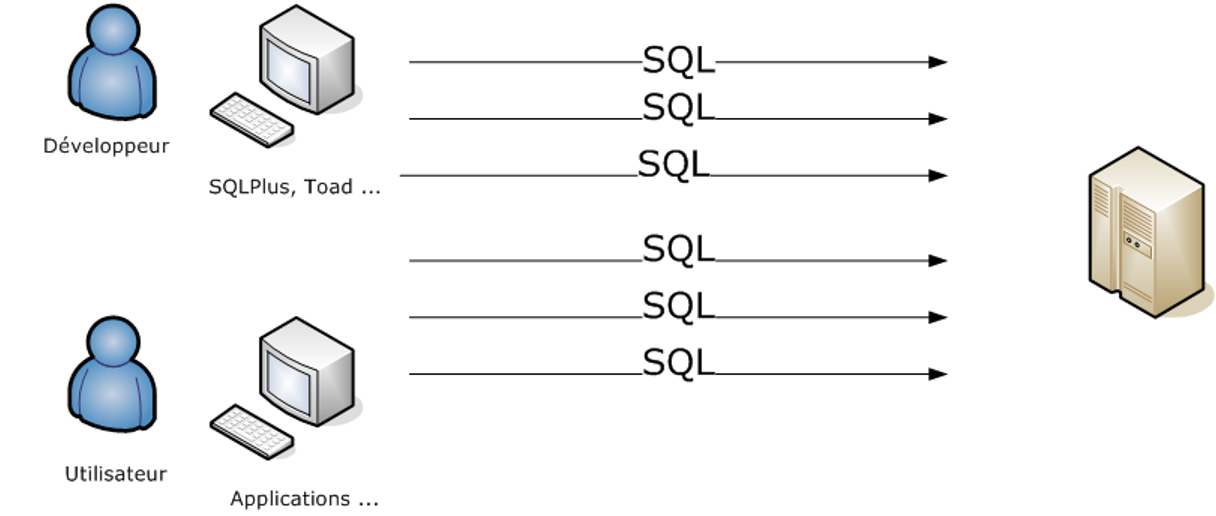
\includegraphics[width=0.9\textwidth]{../assets/img/envoi_instruction.png}
            \caption{Sans PL/SQL : envoi d'instructions SQL}
        \end{center}
    \end{figure}
\end{frame}

\begin{frame}{\secname : \subsecname}
    \begin{figure}
        \begin{center}
            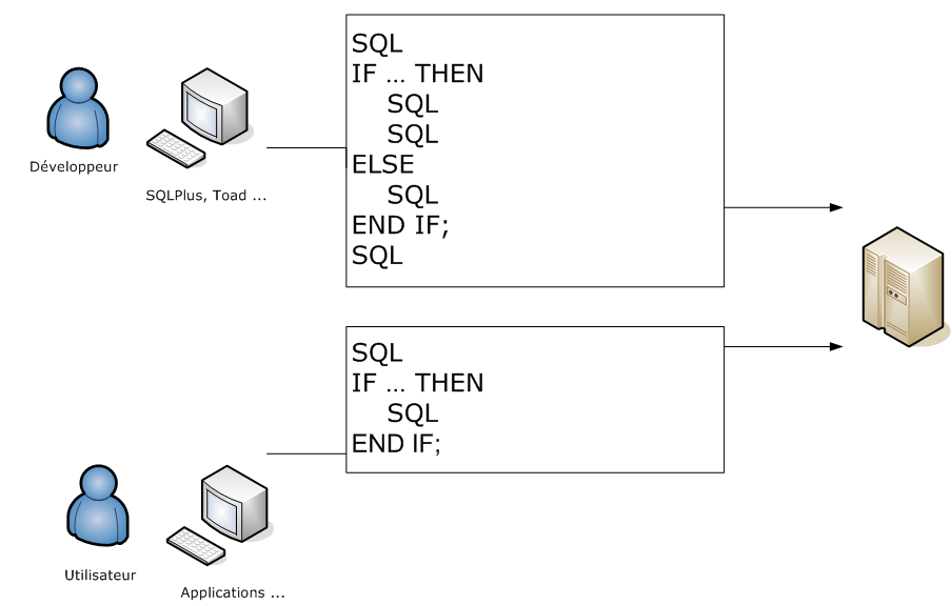
\includegraphics[width=0.9\textwidth]{../assets/img/envoi_instruction-2.png}
            \caption{Avec PL/SQL : écriture de blocs de programmation intégrant SQL}
        \end{center}
    \end{figure}
\end{frame}

\begin{frame}{\secname : \subsecname}
    Une des principales forces du PL/SQL est son intégration avec SQL, surtout au niveau des différents types de données manipulés :
    \begin{itemize}
        \item Une donnée de type \lstinline[language=sql]!DATE! ou \lstinline[language=sql]!VARCHAR! stockée dans la base de données va être stockée dans une variable de même type dans du code PL/SQL
        \item Un instruction de sélection SQL retourne un result set qui peut être défini et exploité en PL/SQL
    \end{itemize}
\end{frame}
\section{Déf de blocs de programmation SQL}
\begin{frame}{\secname}
    \begin{itemize}
        \item Les portions de code PL/SQL peuvent être \textbf{définies dans n'importe quelle interface SQL}
        \item Il suffit d'encoder la portion de code \textbf{comme s}'il s'agissait d'une \textbf{instruction SQL} et de l'exécuter.
        \item Dans cette portion de code, il est possible de réaliser des affichages, d'intercepter des exceptions et de les traiter.
    \end{itemize}
\end{frame}

\begin{frame}{\secname}
    Pour un développeur :
    \begin{itemize}
        \item Programmation SQL dynamique, déclencheurs, méthodes des TAD (types abstraits de données)
        \item Intégration aisée dans les langages classiques OO grâce à sa forte coloration OO
    \end{itemize}
\end{frame}

\begin{frame}{\secname}
    Pour un administrateur, possibilité :
    \begin{itemize}
        \item d'écrire des routines d'administration;
        \item de définir des jobs récurrents,etc.
    \end{itemize}
\end{frame}

\section{Procédures stockées en PL/SQL}
\begin{frame}{\secname}
    \begin{itemize}
        \item PL/SQL permet la création de procédures stockées : terme générique qui signifie qu'une portion de code peut être stockée sur le serveur de base de données dans la base de données elle-même.
        \item Une partie du code peut donc être portée sur le serveur et exécutée par celui-ci. Dans l'architecture classique "client-serveur", le client supporte toute la partie interface (ou présentation) de l'application ainsi que la logique de celle-ci.
    \end{itemize}
\end{frame}

\begin{frame}{\secname}
    \begin{figure}
        \begin{center}
            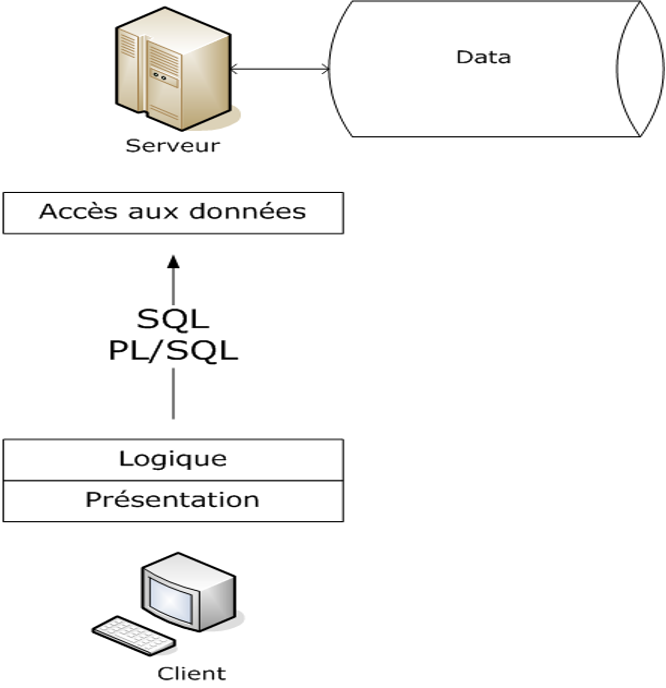
\includegraphics[width=0.6\textwidth]{../assets/img/client_serveur.png}
            \caption{Architecture client-serveur de base}
        \end{center}
    \end{figure}
\end{frame}

\begin{frame}[allowframebreaks]{\secname}
    \begin{figure}
        \begin{center}
            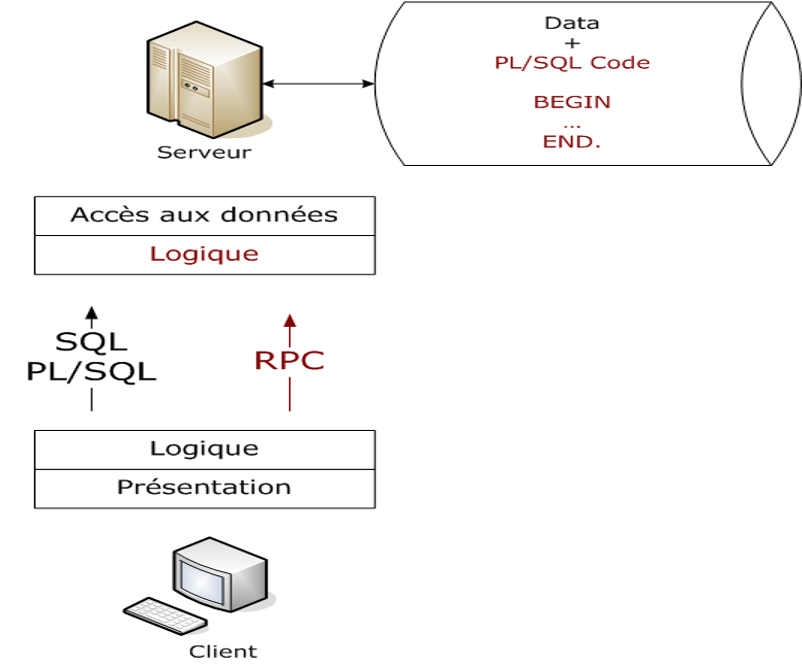
\includegraphics[width=0.6\textwidth]{../assets/img/client_serveur2.png}
            \caption{Les procédures stockées favorisent l'architecture client-serveur de deuxième génération}
        \end{center}
    \end{figure}
    On peut voir sur ce schéma différents avantages :
    \begin{itemize}
        \item  Réutilisabilité : une même procédure ou fonction peut être appelée par plusieurs applications différentes
              Optimisation : le DBA peut utiliser toutes les techniques d'optimisation mises à sa disposition pour les procédures les plus utilisées
        \item Efficacité : une procédure stockée est compilée une fois et stockée sous une forme exécutable.  Les appels peuvent être
        \item efficaces et se font sous forme de RPC (Remote Procedure Call)
    \end{itemize}
\end{frame}

\begin{frame}[allowframebreaks]{\secname}
    En résumé :
    \begin{itemize}
        \item On obtient une \textbf{meilleure performance} et moins de trafic réseau ainsi que de meilleurs temps de réponse
        \item Les procédures stockées font partie de la mémoire cache de la base de données et peuvent être partagées entre les multiples utilisateurs
        \item L'\textbf{indépendance données-programmes s'en trouve renforcée} ! (Les détails du MRD peuvent être cachés aux différents clients.  Il suffit de communiquer au développeur la procédure à appeler ainsi que ses différents paramètres et codes d'erreur)
    \end{itemize}
\end{frame}

\section{Architecture PL/SQL}
\begin{frame}{\secname}
    \begin{itemize}
        \item Le moteur de base de données Oracle coordonne tous les appels en direction de la base de données. \textbf{Le SQL et le PL/SQL comportent chacun un moteur d'exécution associé}.
        \item Lorsqu'un serveur reçoit un appel pour exécuter un programme PL/SQL, \textbf{la version compilée du programme est chargée} en mémoire puis exécutée par les moteurs PL/SQL et SQL.
        \item Le moteur PL/SQL gère les structures en mémoire et le flux logique du programme tandis que le moteur SQL transmet les requêtes à la base de données.
    \end{itemize}
\end{frame}

\begin{frame}{\secname}
    \begin{itemize}
        \item Un code PL/SQL peut être \textbf{appelé} à partir de \textbf{SQL*Plus}, Oracle Forms, Oracle Reports, inclus dans le langage hôte C, C++, Java,...
        \item Dans ce cas, les instructions PL/SQL sont traitées par le moteur PL/SQL embarqué dans l'outil de développement, les \textbf{ordres SQL étant évidemment toujours traités par la base de données}.
    \end{itemize}
\end{frame}

\end{document}